
% The \phantomsection command is needed to create a link to a place in the document that is not a
% figure, equation, table, section, subsection, chapter, etc.
% https://tex.stackexchange.com/questions/44088/when-do-i-need-to-invoke-phantomsection
\phantomsection

% Multiple-language document - babel - selectlanguage vs begin/end{otherlanguage}
% https://tex.stackexchange.com/questions/36526/multiple-language-document-babel-selectlanguage-vs-begin-endotherlanguage
\begin{otherlanguage*}{brazil}

\chapter{Desenvolvimento}

Nesta seção, será abordada a LTI do Beecrowd, que simplifica a integração entre o Moodle e a plataforma Beecrowd. Serão apresentados também os detalhes da implementação da aplicação web do sistema especialista, desenvolvida para auxiliar professores e alunos no esclarecimento de dúvidas recorrentes sobre as questões do Beecrowd, facilitando a adaptação de ambos ao uso da plataforma.

\section{LTI Beecrowd}

Com a disponibilização de uma ferramenta LTI pelo Beecrowd, visando facilitar sua integração com o Moodle, foi elaborado um manual detalhado para orientar o administrador do Moodle na configuração dessa LTI (Apêndice A).

Para configurar uma LTI externa, o administrador deve acessar "Administração do site", selecionar "Plugins" e, em "Módulos de atividade", escolher "Ferramenta externa" e clicar em "Gerenciar ferramentas". Em seguida, deve clicar em "Configurar uma ferramenta manualmente" e preencher os campos conforme as instruções especificadas no Manual de Configuração da LTI Beecrowd no Moodle (Apêndice A). Após a configuração, será possível visualizar os detalhes da ferramenta, os quais deverão ser enviados ao Beecrowd para estabelecer a comunicação entre as plataformas.

Além disso, foi desenvolvido um manual de uso da LTI Beecrowd (Apêndice B), direcionado aos professores que desejam utilizar o Beecrowd como suporte educacional em sala de aula. Esse manual instrui os docentes sobre como criar uma atividade do Beecrowd no Moodle, orientar o acesso dos estudantes e transferir as notas obtidas no Beecrowd para o Moodle.

Após seguir o guia do Manual de Uso da LTI Beecrowd (Apêndice B), duas atividades ficam disponíveis na página do curso, apresentadas como "botões" visuais. A primeira atividade, que é ocultada para os estudantes (Imagem 23), permite ao professor acessar o Beecrowd Academic (Imagem 24) para configurar disciplinas, criar listas de exercícios para os alunos e enviar as notas para o Moodle.

\begin{figure}[H]
    \centering
            \caption{Atividade para o professor acessar o Beecrowd Academic}
            \label{fig:ModeloConceitual}
        
\includegraphics[scale=0.35]{pictures/apendices/apendice_b_5.png}
        \fonte{Produzido pela autora.}
\end{figure}

\begin{figure}[H]
    \centering
            \caption{Beecrowd Academic}
            \label{fig:ModeloConceitual}
        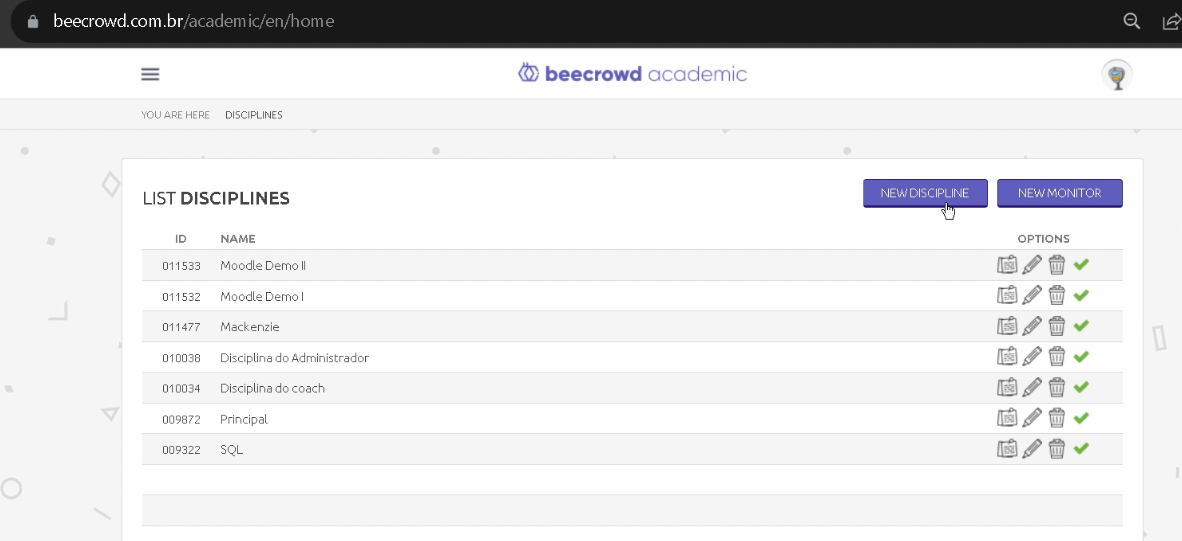
\includegraphics[scale=0.38]{pictures/desenvolvimento/lti_beecrowd_academic.png}
        \fonte{Produzido pela autora.}
\end{figure}

A segunda atividade, acessível aos estudantes (Imagem 25), redireciona-os diretamente para a página no Beecrowd da lista de exercícios criada pelo professor (Imagem 26), sem necessidade de cadastro ou login. Assim, os estudantes podem resolver as atividades diretamente a partir dessa página. Esse botão também permite ao professor acessar a lista de exercícios criada, podendo verificar o progresso dos alunos, as tentativas realizadas e, quando desejado, enviar as notas para o Moodle.

\begin{figure}[H]
    \centering
            \caption{Atividade para o aluno acessar o Beecrowd}
            \label{fig:ModeloConceitual}
        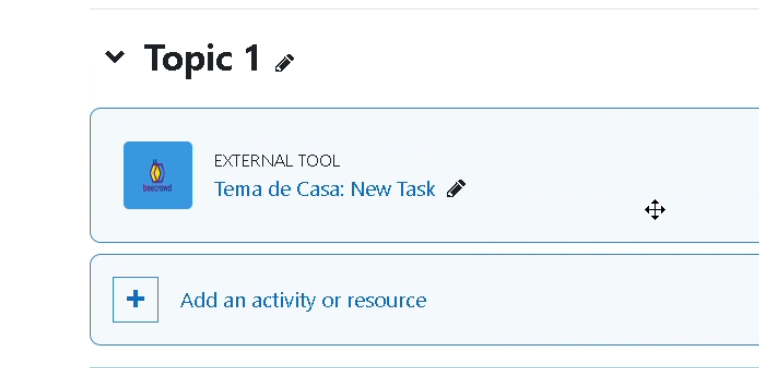
\includegraphics[scale=0.4]{pictures/desenvolvimento/lti_tarefa.png}
        \fonte{Produzido pela autora.}
\end{figure}

\begin{figure}[H]
    \centering
            \caption{Beecrowd do aluno}
            \label{fig:ModeloConceitual}
        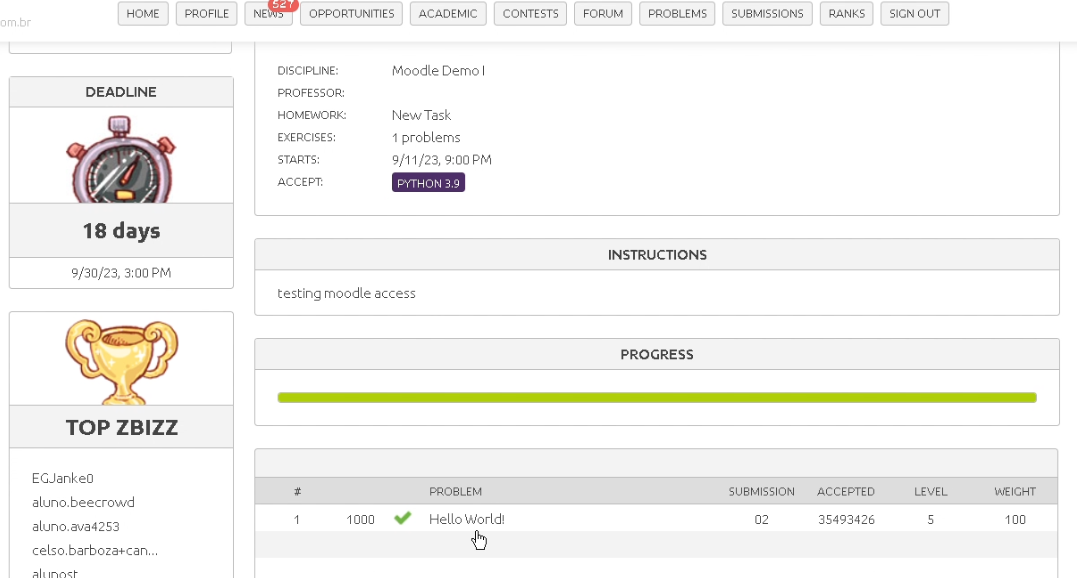
\includegraphics[scale=0.4]{pictures/desenvolvimento/lti_beecrowd_aluno.png}
        \fonte{Produzido pela autora.}
\end{figure}

\section{Sistema Especialista Web}

O objetivo do sistema especialista é oferecer suporte na resolução de dúvidas recorrentes dos estudantes em relação a questões do Beecrowd. A proposta é desenvolver uma aplicação acessível aos alunos via navegador, com um sistema de chat onde o aluno pode informar a questão sobre a qual necessita orientação. O sistema, então, conduz o aluno por meio de perguntas binárias (sim ou não) e, conforme as respostas, fornece dicas relevantes relacionadas ao exercício em questão.

Para viabilizar essa funcionalidade, o sistema especialista será estruturado com um conjunto de dados contendo perguntas direcionadas aos alunos e respostas predefinidas que orientam o aluno na resolução das atividades específicas da disciplina. Em disciplinas como Programação Orientada a Objetos I, onde as listas de exercícios frequentemente incluem questões já utilizadas em semestres anteriores, observa-se uma repetição de problemas e, consequentemente, de dúvidas recorrentes dos alunos.

Assim, a primeira etapa deste trabalho consistiu na coleta de dados sobre as questões, visando identificar e catalogar as dúvidas mais comuns.

\subsection{Coleta de Dados}

Nesta fase, foram realizadas duas coletas de dados: uma com dicas de resolução fornecidas pelo professor para uma lista de exercícios, e outra com as dúvidas dos alunos sobre o uso de listas em Python, com foco em questões específicas.

Na primeira coleta, professor da disciplina de Programação Orientada a Objetos I, da Universidade Federal de Santa Catarina (UFSC), forneceu dicas de resoluções para cada questão de uma lista de exercícios que ainda não tinha sido repassada aos alunos, com o objetivo de avaliar a utilidade da aplicação após ela ser desenvolvida. Assim, quando os alunos fossem resolver a lista de exercícios, poderiam testar a aplicação para ser sua eficácia. As questões abordadas, que receberam as dicas de solução, incluem: 1261, 1281, 1430, 1449, 1483, 1763, 1991, 1953, 2091, 2482, 2492, 2654, 2949 e 2987.

Na segunda coleta, foram registradas as dúvidas dos alunos da disciplina de Programação Orientada a Objetos I, da UFSC, coletadas no dia 30 de outubro de 2024. Nessa data, os alunos estavam trabalhando em uma lista de exercícios sobre o uso de listas em Python. As questões abordadas incluíram os problemas de números 1187, 1435, 1715, 2436, 1383, 1184, 1181 e 1185. Um aspecto notável foi que, durante essa mesma aula, quatro alunos apresentaram a mesma dúvida em relação à questão 1435, especificamente perguntando: "Como resolvo essa questão?"

Durante as 2h30 de aula, a questão 1435 foi a que suscitou o maior número de dúvidas entre os estudantes. Em uma turma de 26 alunos – embora nem todos tenham alcançado essa questão no tempo da aula –, quatro solicitaram uma explicação geral sobre a abordagem para resolvê-la, enquanto dois buscaram orientação sobre a conversão dessa abordagem para o código. Adicionalmente, três alunos enfrentaram o erro "Presentation Error" e um aluno recebeu o erro "Run-time Error".

As dúvidas em relação à questão 1181 refletiram dificuldades comuns no uso de laços de repetição e na manipulação de matrizes. Muitos estudantes não obtinham a resposta correta, mesmo com uma solução aparentemente desenvolvida, devido à confusão na seleção dos elementos da matriz, com erros ao iterar pelas linhas em vez das colunas. Os alunos também enfrentaram dificuldades na estruturação do laço de repetição, especialmente ao calcular a soma dos elementos de uma linha específica e ao determinar o divisor correto para o cálculo da média. Problemas de formatação, que resultaram no erro "Presentation Error", também foram recorrentes, sendo necessário ajustar a saída para uma casa decimal com '%.1f'.

Na questão 1184, as dificuldades estavam relacionadas à estruturação do laço de repetição para percorrer corretamente os elementos abaixo da diagonal principal da matriz. Os alunos foram orientados a usar um laço duplo, com a sequência correta de for i in range(0, 12) e for j in range(0, i). Além disso, houve dúvidas sobre a exclusão dos elementos da diagonal principal, que não deveriam ser somados. Como na questão 1181, os alunos enfrentaram dificuldades de formatação, com orientações para ajustar a saída utilizando '%.1f' para obter uma casa decimal.

As dúvidas relativas à questão 1185 envolveram a manipulação de elementos acima da diagonal secundária da matriz, com os alunos sendo orientados a percorrer as linhas até o último índice da coluna, subtraindo o número da linha. A configuração correta dos laços de repetição foi outra dúvida comum, com muitos alunos invertendo os laços, o que afetou os resultados. A correção do divisor para o cálculo da média e os problemas de formatação também foram pontos críticos, com instruções para usar '%.1f' na saída.

A questão 1187 gerou dúvidas relacionadas aos laços de repetição necessários para somar os elementos da matriz, com os alunos questionando sobre o ajuste dos índices para evitar a soma dos elementos das diagonais. Também surgiram dúvidas sobre como os laços percorriam as linhas e colunas para formar a região triangular desejada, além de questionamentos sobre a lógica para calcular a média e evitar erros de divisão.

A questão 1383, sobre as regras do Sudoku, suscitou dúvidas sobre como validar se uma solução estava correta, além de dificuldades na transformação da lógica para código. A orientação dada foi garantir a não repetição de números em cada linha, coluna, e bloco 3x3, com orientações sobre o uso de depuração com o udebug e Thonny.

A questão 1715 gerou dúvidas sobre a multiplicação dos elementos das linhas para identificar jogadores que marcaram gols em todas as partidas. Os alunos tiveram dificuldades em entender como aplicar esse método corretamente e como garantir que o contador fosse atualizado. A depuração no udebug e Thonny foi útil para a maioria dos alunos, que ajustaram seus códigos após o feedback.

Por fim, a questão 2465 também gerou dúvidas em relação ao uso do comando while True para verificar os vizinhos da matriz. A principal dificuldade foi evitar que o robô retornasse à posição anterior após avançar para um vizinho com valor '1', sendo sugerido que a posição fosse marcada como zero antes de seguir para o próximo vizinho. As orientações permitiram que os alunos avançassem na resolução do problema, superando as dificuldades iniciais.

\subsection{Tecnologias Usadas}

\subsubsection{Prolog e SWI-Prolog}

Para o desenvolvimento do backend da aplicação, utilizou-se a linguagem Prolog, com o auxílio da implementação SWI-Prolog. O SWI-Prolog é uma versão amplamente utilizada do Prolog, que inclui uma série de bibliotecas essenciais para a manipulação de requisições HTTP e dados JSON, como http/thread\_httpd, http/http\_dispatch, http/json, http/http\_session, entre outras. Essas bibliotecas permitem a configuração de um servidor HTTP para o processamento de requisições web e a manipulação de dados JSON. Além disso, elas possibilitam o gerenciamento de sessões, o que viabiliza a integração com aplicações externas e permite o uso simultâneo da aplicação por diferentes usuários \cite{swiprologhttp}.

\subsubsection{API REST}

O servidor definiu os endpoints HTTP (/server e /diagnosis) para o recebimento de requisições POST e GET, permitindo a interação com o backend por meio de uma arquitetura baseada em REST. 

O termo REST (Representational State Transfer) é um estilo de comunicação baseado em padrões e protocolos da web, como HTTP, que permite a troca de dados entre sistemas de forma escalável e eficiente. Nesse modelo, as requisições são realizadas utilizando os métodos HTTP padrão (como GET, POST, PUT e DELETE), facilitando a comunicação entre sistemas de maneira eficiente e escalável \cite{whatisrest}.

\subsubsection{JSON}

JSON (JavaScript Object Notation) é um formato leve e baseado em texto para intercâmbio de dados, independente de linguagem de programação. Derivado do padrão ECMAScript, o JSON define um conjunto simples de regras de formatação para a representação portátil de dados estruturados. Ele busca remover inconsistências com outras especificações e oferece orientações para melhorar a interoperabilidade entre sistemas \cite{whatisjson}.

A biblioteca http/http\_json do SWI-Prolog é utilizada para formatar as respostas no formato JSON, possibilitando que o backend envie dados estruturados para o frontend em um formato amplamente compatível com diversos frameworks web, incluindo o React. Essa abordagem facilita a troca de informações entre o servidor e a interface do usuário, garantindo a interoperabilidade e a eficiência na comunicação entre as camadas da aplicação.

\subsubsection{HTTP e CORS}

CORS (Cross-Origin Resource Sharing) é um mecanismo que permite que requisições do lado do cliente acessem recursos de origens diferentes. Ele define algoritmos que possibilitam que uma API faça requisições a recursos de outra origem, controlando o acesso por meio de cabeçalhos de resposta, como o \textit{Access-Control-Allow-Origin} \cite{whatiscors}.

HTTP (Hypertext Transfer Protocol) é um protocolo de aplicação para sistemas distribuídos e colaborativos de informações hipermídia. É um protocolo genérico e sem estado, utilizado em diversas tarefas além do hipertexto, como servidores de nomes e sistemas de gerenciamento de objetos distribuídos. O HTTP permite a negociação e tipificação da representação dos dados, possibilitando a construção de sistemas independentes dos dados transferidos \cite{whatishttp}.

As bibliotecas http/thread\_httpd, http/http\_dispatch e http/http\_cors, do SWI-Prolog, configuram um servidor HTTP básico, sendo responsáveis pelo tratamento de requisições e respostas. Elas também gerenciam as permissões de CORS, permitindo que o frontend (React) acesse o backend Prolog, mesmo quando este está hospedado em uma origem diferente.

\subsubsection{Sessões HTTP}

Uma sessão HTTP é mantida por meio do uso de cookies, que são pequenos arquivos de dados armazenados nos agentes de usuário (como navegadores) pelos servidores HTTP. Os cabeçalhos Cookie e Set-Cookie permitem que os servidores mantenham o estado de uma sessão, mesmo em um protocolo essencialmente sem estado como o HTTP. Isso significa que, através das sessões, os servidores podem armazenar informações sobre o usuário, como preferências ou dados de autenticação, e usá-las em requisições subsequentes, garantindo uma experiência contínua. Embora os cookies tenham questões históricas relacionadas à segurança e privacidade, os cabeçalhos Cookie e Set-Cookie são amplamente utilizados para gerenciar sessões de usuário, permitindo, por exemplo, o login persistente em sites ou a manutenção de um carrinho de compras em uma loja online \cite{whatissession}.

A biblioteca http/http\_session do SWI-Prolog possibilita o gerenciamento de sessões de usuário, permitindo o armazenamento de variáveis de sessão, como questionNumber e answers. Esse recurso viabiliza a persistência de informações entre requisições subsequentes de um mesmo usuário, assegurando a continuidade do estado da aplicação ao longo da interação.

\subsubsection{React e Typescript (Frontend)}

O frontend foi feito em React\footnote{\url{https://react.dev/}} e Typescript\footnote{\url{https://www.typescriptlang.org/}}, interagindo com o backend por meio de requisições HTTP, acessando endpoints para enviar as respostas do usuário e buscar o resultado final da questão.

React é uma biblioteca para a construção de interfaces de usuário, tanto para a web quanto para aplicativos nativos. Ela permite criar interfaces a partir de unidades individuais chamadas componentes, que podem ser reutilizados e combinados para formar interfaces complexas e interativas. Cada componente em React gerencia seu próprio estado e pode ser renderizado de forma eficiente conforme as mudanças nos dados, facilitando o desenvolvimento de aplicações dinâmicas e de fácil manutenção. React pode ser utilizado com outras linguagens que compilam para JavaScript\footnote{\url{https://www.javascript.com/}}, como TypeScript.

TypeScript é uma linguagem de programação que é um superconjunto do JavaScript, adicionando tipagem estática. Isso permite que os desenvolvedores definam tipos para variáveis e funções, ajudando a identificar erros antes da execução do código. TypeScript melhora a manutenção e segurança do código, especialmente em projetos grandes, e é amplamente utilizado com frameworks como React para criar aplicações mais escaláveis e robustas.

\subsection{Requisitos da Aplicação}

Esta seção descreve os requisitos essenciais para o desenvolvimento da aplicação, divididos em Regras de Negócio, Requisitos Funcionais e Não Funcionais. As Regras de Negócio definem os processos do sistema, enquanto os Requisitos Funcionais especificam as funcionalidades necessárias. Já os Requisitos Não Funcionais tratam de aspectos de qualidade, como desempenho, segurança e arquitetura do sistema.

\subsubsection{Regras de Negócio}

\begin{enumerate}[label=RN\arabic* –]
    \item \textbf{Identificação da Questão}: O usuário deve informar o código da questão do Beecrowd que está tentando resolver para que o sistema possa fornecer dicas específicas.
    \item \textbf{Perguntas Binárias}: O sistema deve formular perguntas binárias (sim/não) para guiar o usuário, baseando-se em possíveis erros ou dificuldades comuns para cada questão.
    \item \textbf{Personalização de Orientações}: Com base nas respostas do usuário, o sistema deve ajustar as perguntas para identificar a dificuldade específica e fornecer a dica mais apropriada.
    \item \textbf{Encerramento do Fluxo}: Ao atingir um número máximo de perguntas, o sistema deve fornecer uma dica final ao usuário.
\end{enumerate}

\subsubsection{Requisitos Funcionais}

\begin{enumerate}[label=RF\arabic* –]
    \item \textbf{Comunicação por Chat}:
    \begin{itemize}
        \item O usuário deve interagir com o sistema por uma interface de chat intuitiva, que apresente respostas sequenciais.
    \end{itemize}

    \item \textbf{Busca e Seleção de Questão}:
    \begin{itemize}
        \item O sistema deve permitir que o usuário informe o código da questão do Beecrowd que deseja resolver.
    \end{itemize}
    
    \item \textbf{Fluxo de Perguntas Binárias}:
    \begin{itemize}
        \item O sistema apresenta perguntas binárias adaptadas conforme as respostas do usuário.
    \end{itemize}

    \item \textbf{Sistema de Dicas}:
    \begin{itemize}
        \item Após a análise das respostas, o sistema deve oferecer dicas relevantes para o problema informado.
    \end{itemize}
\end{enumerate}

\subsubsection{Requisitos Não Funcionais}

\begin{enumerate}[label=RNF\arabic* –]
    \item \textbf{Desempenho}:
    \begin{itemize}
        \item O sistema deve responder em tempo real a cada interação do usuário, mantendo a fluidez do chat.
    \end{itemize}
    
    \item \textbf{Usabilidade}:
    \begin{itemize}
        \item O sistema deve ser intuitivo e fácil de usar, com uma interface de chat amigável.
        \item Deve ser compatível com os principais navegadores modernos.
    \end{itemize}

    \item \textbf{Escalabilidade}:
    \begin{itemize}
        \item O sistema deve suportar o uso simultâneo de múltiplos usuários.
    \end{itemize}
    
    \item \textbf{Segurança}:
    \begin{itemize}
        \item As sessões de chat devem ser isoladas, para evitar vazamento de informações entre os usuários.
    \end{itemize}
    
    \item \textbf{Manutenibilidade}:
    \begin{itemize}
        \item O sistema deve ter um código modular, facilitando a inclusão de novas perguntas e dicas para futuras questões do Beecrowd.
    \end{itemize}
    
    \item \textbf{Arquitetura Backend e Frontend}:
    \begin{itemize}
        \item O sistema deve ter um backend desenvolvido em Prolog, utilizando SWI-Prolog para lidar com requisições HTTP.
        \item O backend deve definir configurações de CORS apropriadas para permitir a comunicação entre cliente e servidor.
        \item O backend deve seguir o padrão de API REST e devolver respostas no formato JSON.
        \item O backend deve conter o sistema especialista, que processa as perguntas e respostas para oferecer suporte aos estudantes.
        \item O frontend deve ser desenvolvido em React e TypeScript, proporcionando uma interface interativa e amigável para os alunos.
    \end{itemize}
\end{enumerate}

\subsection{Arquitetura de Software}

A aplicação propõe uma interação dinâmica em que o usuário, ao informar o número da questão sobre a qual deseja obter orientações, inicia um diálogo com o sistema de chat. O chat responde com perguntas específicas para compreender melhor as necessidades do usuário, permitindo direcionar as orientações de forma mais precisa. Conforme o usuário responde com "sim" ou "não" a cada pergunta, o sistema adapta as próximas questões e sugestões, guiando-o progressivamente até fornecer uma orientação final ajustada ao contexto das respostas acumuladas.

A Figura 27 apresenta o diagrama de atividades que detalha o fluxo de interação entre o usuário e o chat da aplicação. Após informar o número da questão sobre a qual deseja obter orientações, o usuário recebe uma pergunta inicial, respondendo com "sim" ou "não". Se houver mais perguntas, o chat continua a apresentá-las até que todas sejam respondidas, conduzindo o usuário a uma orientação final baseada nas respostas acumuladas. Ao final, o usuário pode iniciar o processo novamente com outro número de questão ou com o mesmo, caso deseje explorar outras sugestões e perguntas relacionadas.

\begin{figure}[h!]
    \centering
            \caption{Diagrama de Atividades do Usuário da Aplicação}
            \label{fig:ModeloConceitual}
        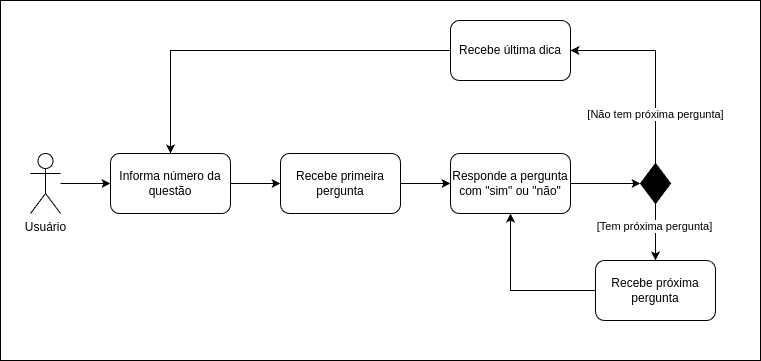
\includegraphics[scale=0.6]{pictures/atividade1.png}
        \fonte{Produzido pela autora.}
\end{figure}

A Figura 28 representa a estrutura da aplicação, mostrando a interação entre o frontend e o backend através de requisições. No frontend, o arquivo \textit{ActionProvider.tsx} gerencia as mensagens enviadas pelo usuário no chat, processando tanto o número da questão informada, quanto as respostas de "sim" ou "não". Por meio dessas requisições, o \textit{frontend} envia esses dados ao \textit{backend}, que, em resposta, fornece perguntas e dicas relacionadas à questão solicitada. Caso o usuário peça uma nova dica e o \textit{backend} não tenha mais sugestões para aquela questão, ele envia a orientação final da questão, que é então apresentada ao usuário.

\begin{figure}[h!]
    \centering
            \caption{Arquitetura da Aplicação do Sistema Especialista}
            \label{fig:ModeloConceitual}
        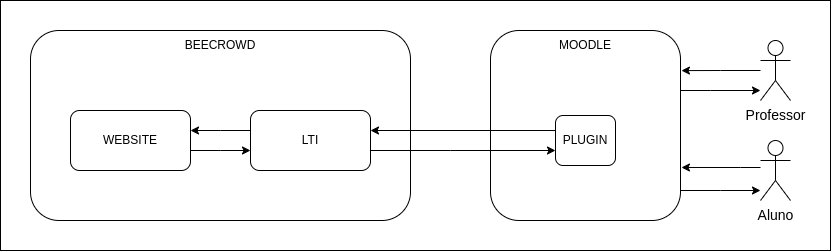
\includegraphics[scale=0.6]{pictures/arquitetura.png}
        \fonte{Produzido pela autora.}
\end{figure}


\subsection{Comunicação Frontend-Backend}

O Código 1 representa como o arquivo \textit{ActionProvider.tsx} informa para o backend o número da questão. Ele define duas funções assíncronas: \texttt{fetchData} e \texttt{handleFirstMessage}, usadas para interagir com um \textit{backend} via requisições HTTP. A função \texttt{fetchData} recebe uma URL e um corpo de dados (\texttt{URLSearchParams}) para fazer uma requisição \texttt{POST}. Ela define cabeçalhos para enviar os dados como \texttt{application/x-www-form-urlencoded}, garantindo que o backend receba os dados em um formato compatível e de fácil manipulação, especialmente em linguagens que interpretam parâmetros de URL de forma nativa. Além disso, a função inclui cookies nas requisições com \texttt{credentials: 'include'} para permitir que a sessão seja mantida entre as requisições, o que é crucial para a continuidade da comunicação com o backend. Caso a resposta não tenha o status 200, a função trata o erro, retornando uma mensagem de erro em vez do JSON da resposta. 

A função \texttt{handleFirstMessage} constrói um corpo de dados contendo \texttt{questionNumber} e chama \texttt{fetchData} para enviar esses dados ao \textit{backend} no endpoint \texttt{"http://localhost:6358/server"}. Em seguida, cria uma estrutura de mensagens adicionais vazia e invoca \texttt{handleMessageResponse} para manipular a resposta, preenchendo essa estrutura conforme a resposta recebida.

\begin{lstlisting}[style=ufscthesisx_style, caption={Funções assíncronas para requisição HTTP}]
    const fetchData = async (url: string, body: URLSearchParams) => {
        try {
            const response = await fetch(url, {
            method: "POST",
            headers: { 'Content-Type': 'application/x-www-form-urlencoded;charset=UTF-8' },
            credentials: 'include',
            body,
            });
    
            if (response.status !== 200) throw new Error("Erro ao consultar o backend.");
    
            return await response.json();
        } catch (error) {
            return { error: "Erro ao consultar o backend." };
        }
    };

const handleFirstMessage = async (questionNumber?: string) => {
    const body = new URLSearchParams({ questionNumber: questionNumber?.toString() || '' });
    const data = await fetchData("http://localhost:6358/server", body);
    let additionalMessages: {
        messages: {
        message: string;
        type: string;
        id: number;
        loading?: boolean;
        widget?: string | undefined;
        delay?: number | undefined;
        payload?: any;
        }[];
    }[] = [];

    await handleMessageResponse(data, additionalMessages);
};
\end{lstlisting}

\subsection{Elementos do Backend}

Pela Figura 28 também observa-se que o \textit{backend} é composto pelo arquivo principal \textit{server.pl} e por arquivos específicos para cada questão, nomeados no formato \textit{questao\_\{numeroDaQuestao\}.pl}, onde cada um contém dicas voltadas para uma questão particular. Por exemplo, o arquivo \textit{questao\_1234.pl} armazena as orientações para a questão 1234 do Beecrowd.

\subsubsection{Arquivos no formato questao\_\{numeroDaQuestao\}.pl}

O Código 2 apresenta o arquivo \textit{questao\_1181.pl} como um exemplo de estrutura para arquivos do tipo \textit{questao\_\{numeroDaQuestao\}.pl}.

\begin{lstlisting}[style=ufscthesisx_style, caption={Arquivo \textit{questao\_1181.pl}}]
    :- module(questao_1181, [questao/3, diagnostico/3]).
    
    % Predicado para fornecer perguntas com base na sequência de respostas
    questao(1181, [], "Você já desenvolveu sua solução, mas não está saíndo a resposta correta?").
    questao(1181, ["sim"], "Tome cuidado que a questão quer todos os elementos da linha, e não da coluna! Verifique \ccomo você está iterando sobre a matriz: se está pegando todos os elementos de uma linha \c ou todos os elementos de uma coluna. Mais uma dica sobre isso?").
    questao(1181, ["sim", "sim"], "Se sua matriz é feita de forma que é iterada assim: matriz[linha][coluna], verifique \cse o 'for' está correto. Quer saber como o for fica?").
    questao(1181, ["sim", "sim", "sim"], "considerando que l é a entrada do usuário que indica a linha que será a \cconsiderada para operação: \nfor i in range(0, 12): soma += matriz[l][i]. \n\cPróxima dica?").
    questao(1181, ["sim", "sim", "sim", "sim"], "Verifique se o número pelo qual você está tentando dividir para \cpara conseguir a média está correto. Próxima pergunta?").
    
    
    questao(1181, Respostas, "Deu Presentation Error?") :-
        Respostas = ["não"];
        Respostas = ["sim", "não"];
        Respostas = ["sim", "sim", "não"];
        Respostas = ["sim", "sim", "sim", "não"];
        Respostas = ["sim", "sim", "sim", "sim", "sim"].
    
    questao(1181, Respostas, "Perceba que a formatação que a questão pede é: Imprima o resultado solicitado \c(a soma ou média), com 1 casa após o ponto decimal. Ou seja, '%.1f'. Deu certo?") :-
        Respostas = ["não", "sim"];
        Respostas = ["sim", "não", "sim"];
        Respostas = ["sim", "sim", "não", "sim"];
        Respostas = ["sim", "sim", "sim", "não", "sim"];
        Respostas = ["sim", "sim", "sim", "sim", "sim", "sim"].
    
    
    % Diagnóstico com base nas respostas completas
    diagnostico(1181, Respostas, "Legal! Parabéns!") :-
        Respostas = ["não", "sim", "sim"];
        Respostas = ["sim", "não", "sim", "sim"];
        Respostas = ["sim", "sim", "não", "sim", "sim"];
        Respostas = ["sim", "sim", "sim", "não", "sim", "sim"];
        Respostas = ["sim", "sim", "sim", "sim", "não", "sim", "sim"].
    
    diagnostico(1181, _, "Atente-se bem às dicas já enviadas ou pergunte novamente! Além disso, você pode \cusar o udebug para verificar a diferença entre as saídas do seu código, e as \csaídas esperadas pela questão! Também é uma boa ideia debugar seu código no Thonny, \crevisando linha por linha, ou usando prints para entender o que ele está executando!").
\end{lstlisting}    

Esse arquivo Prolog define um módulo especializado para auxiliar usuários na resolução da questão 1181 por meio de um sistema especialista baseado em regras. O módulo \textit{questao\_1181} implementa dois predicados principais: \textit{questao/3} e \textit{diagnostico/3}, que são responsáveis por operacionalizar a lógica de suporte do sistema.

\begin{itemize}
    \item \textbf{Predicado \textit{questao/3}:} Este predicado orienta o usuário de maneira sequencial, adaptando as instruções com base nas respostas fornecidas. Ele recebe três parâmetros: o identificador da questão, uma lista de respostas (que mantém o histórico de interações), e uma mensagem de orientação. A matriz de decisões, implementada neste predicado, direciona o fluxo de perguntas e respostas com base no histórico de interações do usuário, promovendo uma progressão lógica que facilita a resolução da questão. Essa matriz está estruturada de forma que cada combinação de respostas leva a uma nova instrução, que oferece dicas cada vez mais específicas até que o usuário obtenha a solução correta.

    A tabela 2 apresenta a matriz de decisões para o predicado \textit{questao/3}, em formato de tabela, representando as combinações de respostas possíveis e as respectivas instruções emitidas:

    \begin{longtable}{|c|p{5cm}|p{8cm}|}
        \caption{Matriz de Decisões para o Predicado \textit{questao/3} na Questão 1181} \\
        \hline
        \textbf{Questão} & \textbf{Respostas} & \textbf{Instrução} \\
        \hline
        \endfirsthead
        \multicolumn{3}{|c|}{\textbf{Continuação da Tabela}} \\
        \hline
        \textbf{Questão} & \textbf{Respostas} & \textbf{Instrução} \\
        \hline
        \endhead
        \hline
        \endfoot
        \hline
        \endlastfoot
        
        1181 & [] & Você já desenvolveu sua solução, mas não está saindo a resposta correta? \\
        \hline
        1181 & [sim] & Tome cuidado que a questão quer todos os elementos da linha, e não da coluna! Verifique como você está iterando sobre a matriz: se está pegando todos os elementos de uma linha ou todos os elementos de uma coluna. Mais uma dica sobre isso? \\
        \hline
        1181 & [sim, sim] & Se sua matriz é feita de forma que é iterada assim: matriz[linha][coluna], verifique se o 'for' está correto. Quer saber como o for fica? \\
        \hline
        1181 & [sim, sim, sim] & Considerando que l é a entrada do usuário que indica a linha que será considerada para operação: \texttt{for i in range(0, 12): soma += matriz[l][i]} \newline Próxima dica? \\
        \hline
        1181 & [sim, sim, sim, sim] & Verifique se o número pelo qual você está tentando dividir para calcular a média está correto. Próxima pergunta? \\
        \hline
        1181 & [não], [sim, não], [sim, sim, não], [sim, sim, sim, não], [sim, sim, sim, sim, sim] & Deu Presentation Error? \\
        \hline
        1181 & [não, sim], [sim, não, sim], [sim, sim, não, sim], [sim, sim, sim, não, sim], [sim, sim, sim, sim, sim, sim] & Perceba que a formatação que a questão pede é: Imprima o resultado solicitado (a soma ou média), com 1 casa após o ponto decimal. Ou seja, \%.1f. Deu certo? \\
      \end{longtable}
    
    \item \textbf{Predicado \textit{diagnostico/3}:} Este predicado fornece um diagnóstico final com base nas respostas acumuladas ao longo da interação. Atuando como feedback conclusivo, ele emite uma mensagem de sucesso caso as respostas indiquem que o usuário compreendeu e solucionou a questão. Caso contrário, sugere ferramentas como o \textit{udebug} e o depurador \textit{Thonny}, de modo que o usuário possa inspecionar o comportamento do seu código em detalhes.
\end{itemize}

Dessa forma, arquivos do formato \textit{questao\_\{numeroDaQuestao\}.pl} devem seguir essa estrutura, onde cada questão contém um predicado \textit{questao/3} para fornecer orientações sequenciais e um predicado \textit{diagnostico/3} para avaliação final. A matriz de decisões implementada no predicado \textit{questao/3} permite um processo dinâmico e adaptativo de interação, guiando o usuário de forma direcionada e progressiva na resolução da questão específica.

\subsubsection{Arquivo server.pl}

\subsubsubsection{Configurando servidor HTTP}

O arquivo \textit{server.pl} configura e inicializa um servidor HTTP, definindo rotas para processar requisições e habilitando o CORS, permitindo conexões da porta do \textit{frontend}. Ele recebe requisições \textit{POST} para iniciar ou continuar uma questão, associando cada sessão ao usuário correspondente, e também aceita requisições \textit{GET} para fornecer o diagnóstico final com base nas respostas acumuladas durante a interação.

O Código 3 exemplifica a configuração de um servidor HTTP em Prolog utilizando o módulo \texttt{http\_dispatch}, no qual as rotas são definidas por meio de \texttt{http\_handler} para manipular requisições \textit{GET}, \textit{POST} e \textit{OPTIONS}. Especificamente, a requisição \textit{POST} é tratada pela rota \texttt{server}, sendo manipulada pela função \texttt{handle\_post\_request}.

\begin{lstlisting}[style=ufscthesisx_style, caption={Arquivo \textit{server.pl} - \textit{Handlers} e Manipuladores de requisições}]
% Define o handler para receber as requisições HTTP POST
:- http_handler(root(server), handle_post_request, [method(post)]).
:- http_handler(root(.), handle_options, [method(options)]).

% Manipulador de requisições POST
handle_post_request(Request) :-
    member(method(post), Request), !,
    
    % Garante que a sessão está ativa para o cliente
    http_session_id(_SessionID),

    % Lê os dados da requisição
    http_read_data(Request, Data, [encoding(utf8)]),

    % Definindo os headers para permitir CORS
    format('Access-Control-Allow-Origin: http://localhost:5173~n'),
    format('Access-Control-Allow-Credentials: true~n'),
    format('Content-Type: application/json; charset=UTF-8'),
    cors_enable(Request, [methods([post])]),

    (   % Caso seja a primeira requisição da questão
        member(questionNumber=QN, Data) 
    ->  % Inicializa a sessão e a questão
        http_session_retractall(questionNumber(_)),
        http_session_retractall(answers("Answers", _)),
        http_session_assert(answers("Answers", [])),
        
        http_session_assert(questionNumber(QN)),
        start_question(QN, FirstQuestion),

        reply_json_dict(FirstQuestion)

    ;   % Caso receba respostas subsequentes
        member(answer=Answer, Data),
        
        % Garante que a sessão tenha a variável questionNumber
        ( http_session_data(questionNumber(QN)) ->
            continue_question(QN, Answer, NextQuestionOrResult),
            reply_json_dict(NextQuestionOrResult)
        ;   % Erro caso a sessão não tenha um questionNumber
            reply_json_dict(_{error: "Número da questão não encontrado na sessão"})
        )
    ).
\end{lstlisting}    

O \textbf{manipulador de requisições POST} (\texttt{handle\_post\_request}) tem como função processar requisições \textit{POST} enviadas ao servidor, gerenciando o fluxo de perguntas e respostas entre o cliente e o servidor. Inicialmente, ele habilita o CORS, permitindo requisições provenientes do frontend no endereço \texttt{http://localhost:5173}, além de configurar os cabeçalhos necessários para o envio de credenciais, como cookies de sessão. A função verifica se a sessão está ativa, garantindo a associação com um ID de sessão único.

Dependendo do tipo de requisição, a função processa a primeira pergunta ou continua a sequência de perguntas baseadas nas respostas anteriores. Se for a primeira requisição, o número da questão é extraído, e a sessão é inicializada com os dados necessários. Além disso, o arquivo correspondente à questão é carregado dinamicamente. 

Caso seja uma resposta subsequente, a função valida a presença do número da questão na sessão, atualiza as respostas e retorna a próxima pergunta ou o resultado final. Se os dados da sessão estiverem faltando, um erro é enviado indicando que o número da questão não foi encontrado.

\subsubsubsection{Carregando os arquivos das questões}

Os arquivos de questões são carregados dinamicamente no \textit{server.pl} com base no número da questão recebido nas requisições \textit{POST}. Se o usuário alterna para uma nova questão, por exemplo, a questão Y, o \textit{backend} carrega o arquivo \textit{questao\_Y.pl} e passa a conduzir a interação de acordo com suas informações. 

No Código 4, é mostrado o trecho do \texttt{server.pl} que realiza esse carregamento dinâmico. O predicado \texttt{start\_question/2} tem como objetivo inicializar uma nova questão dentro de um sistema interativo, baseado no número da questão fornecido. O primeiro passo do código é construir o caminho para o arquivo que contém a definição da questão, concatenando o prefixo \texttt{questao\_} com o número da questão \texttt{(QuestionNumber)} e adicionando a extensão \texttt{.pl} para formar o nome completo do arquivo. Isso é realizado através do predicado \texttt{atom\_concat\/3}, que concatena átomos (strings) para formar o caminho completo do arquivo a ser carregado.

\begin{lstlisting}[style=ufscthesisx_style, caption={Arquivo \textit{server.pl} - \textit{Handlers} e Manipuladores de requisições}]
start_question(QuestionNumber, FirstQuestion) :-
    atom_concat('questao_', QuestionNumber, FileName),
    atom_concat(FileName, '.pl', FilePath),

    % Verifica se o arquivo existe antes de tentar carregá-lo
    (   exists_file(FilePath)
    ->  % Carrega dinamicamente o arquivo da questão
        abolish(questao/3),
        abolish(diagnostico/3),

        ensure_loaded(FilePath)
    ).
\end{lstlisting}

Depois, o código verifica se o arquivo gerado existe no sistema de arquivos utilizando o predicado \texttt{exists\_file\/1}. Caso o arquivo exista, o sistema prossegue para carregá-lo dinamicamente com o predicado \texttt{ensure\_loaded\/1}. Antes de carregar o arquivo, o predicado \texttt{abolish\/1} é utilizado para garantir que qualquer definição anterior dos predicados \texttt{questao\/3} e \texttt{diagnostico\/3} seja removida da memória, evitando conflitos ou sobrecarga de definições antigas.

\subsubsubsection{Recebe respostas}

O arquivo \textit{server.pl} também armazena na sessão do usuário as informações fornecidas, como número da questão e respostas, para garantir a continuidade da interação. O Código 5 apresenta a função \textbf{continue\_question}, responsável por processar respostas subsequentes enviadas pelo usuário para uma questão em andamento, armazenando a resposta na sessão e determinando o próximo passo com base nas respostas acumuladas. Inicialmente, a função adiciona a nova resposta à lista de respostas da sessão, atualizando a variável de sessão \texttt{answers("Answers")}. Em seguida, tenta gerar a próxima pergunta por meio da chamada ao predicado \texttt{questao/3}. Se \texttt{questao/3} retornar uma nova pergunta (\texttt{NextQuestion}), esta é enviada ao cliente para dar continuidade à interação. Caso contrário, a função verifica se uma resposta final pode ser gerada utilizando o predicado \texttt{diagnostico/3}. O resultado final, seja uma nova pergunta ou uma conclusão, é então enviado ao cliente no formato JSON, permitindo que a interação prossiga ou seja concluída de acordo com o progresso da sessão.

\begin{lstlisting}[style=ufscthesisx_style, caption={Arquivo \textit{server.pl} - \textit{Handlers} e Manipuladores de requisições}]
continue_question(QuestionNumber, Answer, Response) :-
    (   string(Answer) -> AW = Answer
    ;   atom(Answer) -> atom_string(Answer, AW)
    ;   term_string(Answer, AW)
    ),
    atom_number(QuestionNumber, QN), 

    % Salva a resposta na sessão
    http_session_data(answers("Answers", AnswerList)),
    append(AnswerList, [AW], UpdatedAnswers),
    http_session_retractall(answers("Answers", _)),
    http_session_assert(answers("Answers", UpdatedAnswers)),

    % Chama a questão correspondente com a lista atualizada de respostas
    (   questao(QN, UpdatedAnswers, NextQuestion)
    ->  Response = _{question: NextQuestion}
    ;   (   diagnostico(QN, UpdatedAnswers, Result)
        ->  true
        ;   Result = "Sem conclusão final."
        ),
        Response = _{result: Result}
    ).

\end{lstlisting}

\subsection{Elementos do Frontend}

\end{otherlanguage*}

